%%%%%%%%%%%%%%%%%%%%%%%%%%%%%%%%%%%%%%%%%%%%%%%%%%%%%%%%%%%%%%%
\section{Tracks and primary vertices}\label{sec:tracksandvtx}
%%%%%%%%%%%%%%%%%%%%%%%%%%%%%%%%%%%%%%%%%%%%%%%%%%%%%%%%%%%%%%%

The reconstruction of tracks of charged particles in a magnetic field allows for their momentum measurement and aids in particle identification as described in subsequent sections. The reconstruction of the tracks' vertices is important to distinguish the primary interaction, i.e. the hard interaction, from additional interactions that might take place in the event and also for the identification of secondary vertices in jets that contain c or b quarks called c/b tagging (see Sec.~\ref{subsec:bjets}).

%%%%%%
\subsection{Track reconstruction}\label{subsec:tracks}
%%%%%%

The track reconstruction at CMS~\cite{Chatrchyan:2014fea} is based on information coming from the silicon tracker system. A charged particle passing through a tracker layer can in general induce a signal in more than one pixel or more than one strip. The first step of the tracking procedure is the assembly of nearby tracker channels into one hit cluster. The particle position and its uncertainty is then inferred from the relative signal amplitudes in each channel.
%Despite the good performances and resolutions of the detectors, the track reconstruction is challenging due to the high density of tracks, to the presence of additional pileup vertices in each bunch crossing and to the amount of detector material leading to multiple scattering, energy loss and nuclear interactions.

Because of the magnetic field, charged particles travel through the tracking detectors on a helical trajectory which is described by 5 parameters: the curvature $k$, the track azimuthal angle $\phi$ and polar angle $\theta$, the signed transverse impact parameter $d_0$ and the longitudinal impact parameter $z_0$. The transverse (longitudinal) impact parameter of a track is defined as the transverse (longitudinal) distance of closest approach of the track to the primary vertex.

The trajectories of charged particles are reconstructed through an iterative procedure consisting of multiple iterations of the \textit{Combinatorial Track Finder algorithm} (CTF)~\cite{Adam:934067}, which uses the reconstructed hits in the silicon detectors to determine the track parameters. In the first iterations the algorithm searches for tracks of relative large \pt and produced near the interaction region. Then, hits associated to high quality tracks are iteratively removed from the input list to reduce the combinatorial complexity of the next iterations, and to allow the more difficult reconstruction of low \pt or displaced tracks. Each iteration of the CTF algorithm is made of three steps: track seeding, track finding and track fitting.

In the first step, a first estimate of the helix parameters and of its covariance matrix is provided using only pairs or triplets of hits compatible with the hypothesis of a track coming from the pp interaction region. Track candidates are best seeded from hits in the pixel detector because of the low occupancy, high efficiency and unambiguous 3-dimensional position information.

The track finding stage associates new hits in the next tracker layers to the trajectory obtained from seeds using a standard Kalman Filter (KF) pattern recognition approach~\cite{Billoir:1989mh,Fruhwirth:1987fm}, which takes into account the effect of multiple scattering in the tracker layers. The current trajectory is extrapolated to the next tracker layer and compatible hits are assigned to the track on the basis of the $\chi^2$ between the predicted and measured positions. In case multiple compatible hits are found when extrapolating the helix to a single layer, the algorithm creates one trajectory candidate for each hit and they are propagated independently. Furthermore, in order to take into account possible inefficiencies, one additional candidate is created without including any hit information. A quality index is assigned to the tracks, based on the $\chi^2$, the number of missing hits, and how compatible they are with originating from a primary interaction vertex. Only the best quality tracks are kept for further propagation and ambiguities are resolved between tracks during and after track finding. In case two tracks share more than 50\% of their hits, the lower quality track is discarded. The fake rate, defined as the fraction of reconstructed tracks not associated with a charged particle, is substantially reduced by these quality requirements.

For each trajectory the finding stage results in an estimate of the track parameters. However, since the full information is only available at the last hit and constraints applied during trajectory building can bias the estimate of the track parameters, all valid tracks are refitted using the KF to determine the most accurate estimate of the helix parameters. The usual fit starting from the interaction point to the end of the tracker is complemented with a second fit running backward from the outermost tracker layer to the interaction point. The second fit is found to improve the accuracy of the \pt and impact parameter measurement by 0.5\% and 1\%, respectively.\\

%Figure~\ref{fig:track_eff} shows the tracking reconstruction efficiency as a function of $\eta$ for simulated muons, electrons, and pions.
%The tracking reconstruction efficiency has been measured to be $> 99\%$ for the isolated muons with $1 < \pt < 100\GeV$ in the $|\eta| < 2.5$ range, from 98\% to 89\% for 10\GeV pions and over 92\% for $>10\GeV$ electrons, as shown in Fig.~\ref{fig:track_eff}. 
The performance of the track reconstruction is shown in Fig.~\ref{fig:track_eff} for simulated muons, electrons and pions.
For isolated muons with $1 < \pt < 100\GeV$, the track reconstruction efficiency is $>$ 99\% over the full $\eta$-range of tracker acceptance, and does not depend on \pt (Fig.~\ref{fig:track_eff_a}). The fake rate is completely negligible. For pions and electrons the efficiency is in general lower along with a higher fake rate because of interactions with the material in the tracker. The material budget of the CMS tracker in units of radiation length is presented in Fig.~\ref{fig:budgetCMStracker}. By comparing this distribution with the tracking efficiencies presented in Fig.~\ref{fig:track_eff}, it can be noticed that the efficiency for electrons and pions are significantly reduced in correspondence of the regions of the detector with the highest material budget.

\begin{figure}[!htb]
\centering
\subfigure[]{\label{fig:track_eff_a}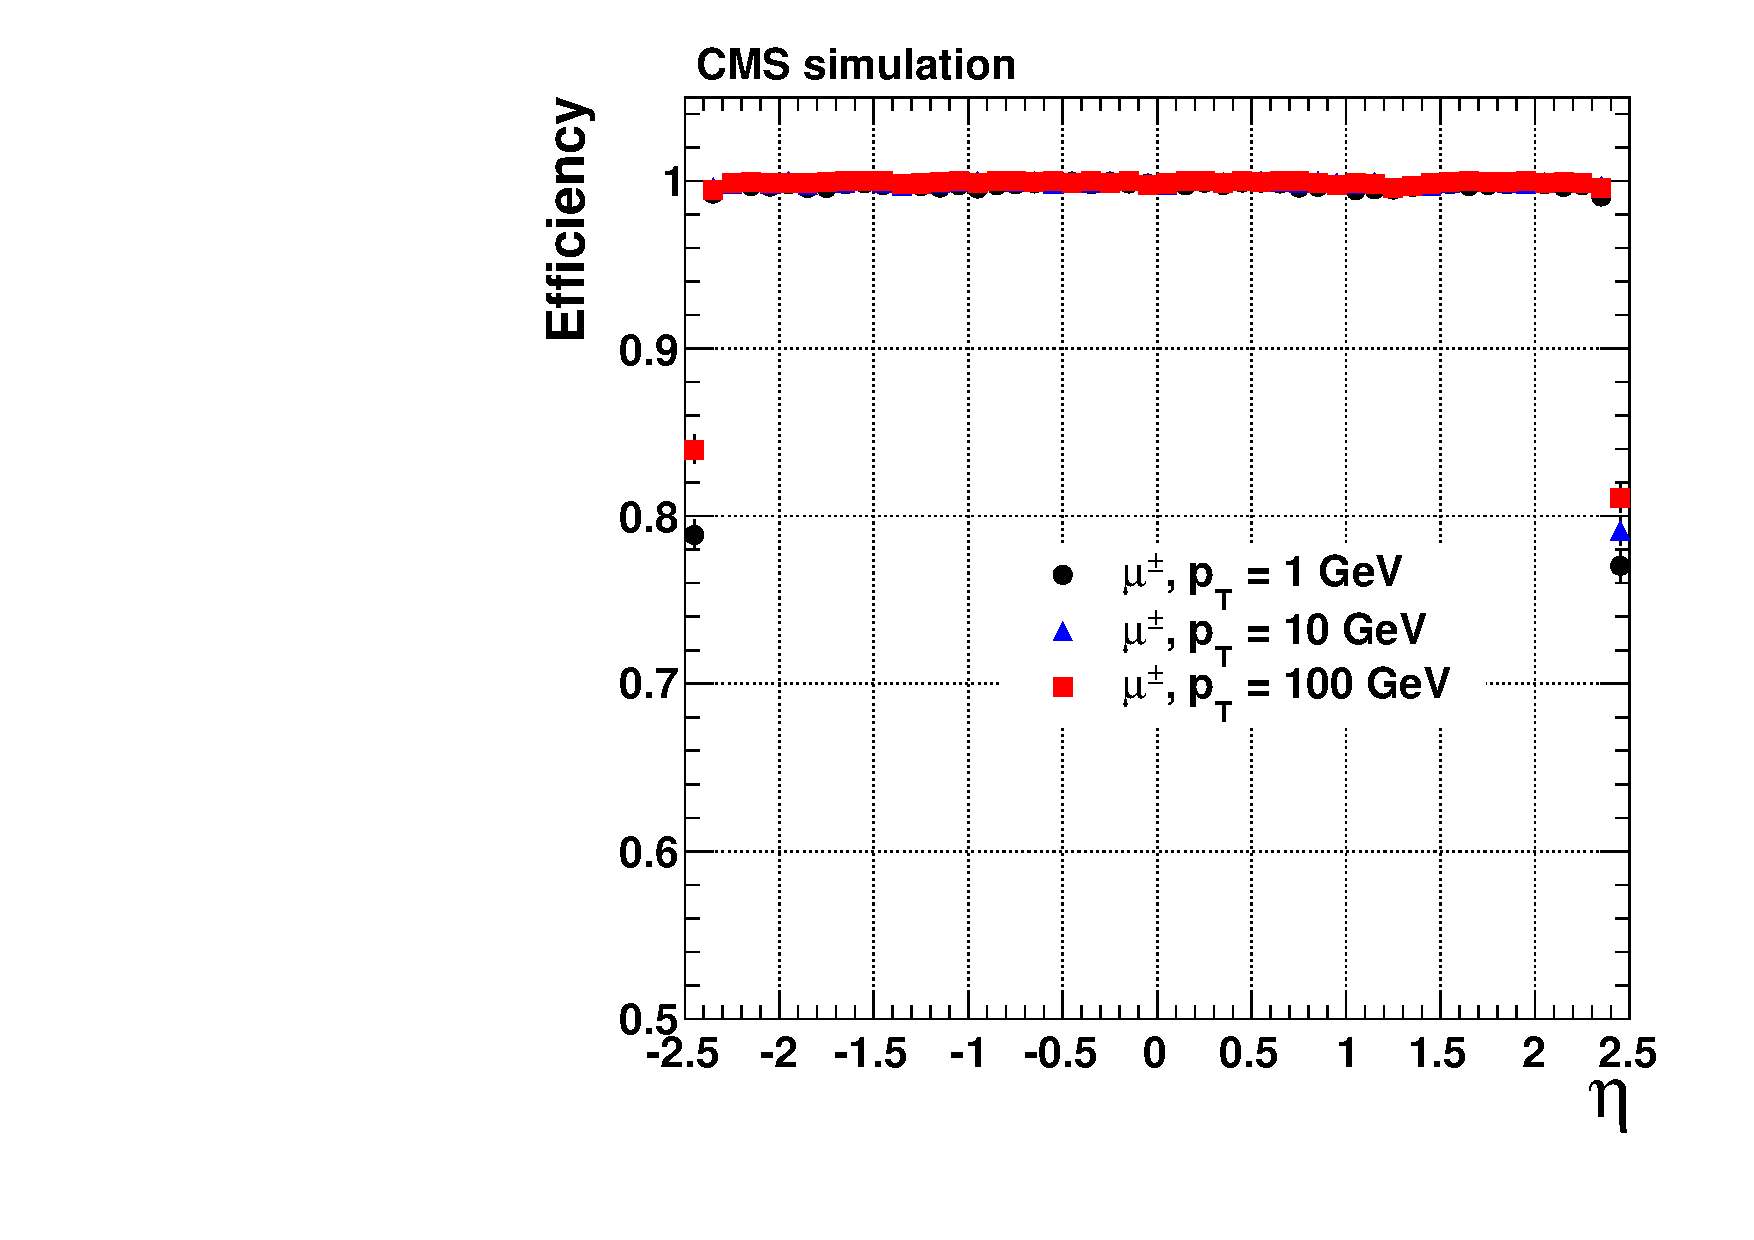
\includegraphics[width=0.30\textwidth]{\chsix/mu-efficiencyVsEta.pdf}}
\subfigure[]{\label{fig:track_eff_b}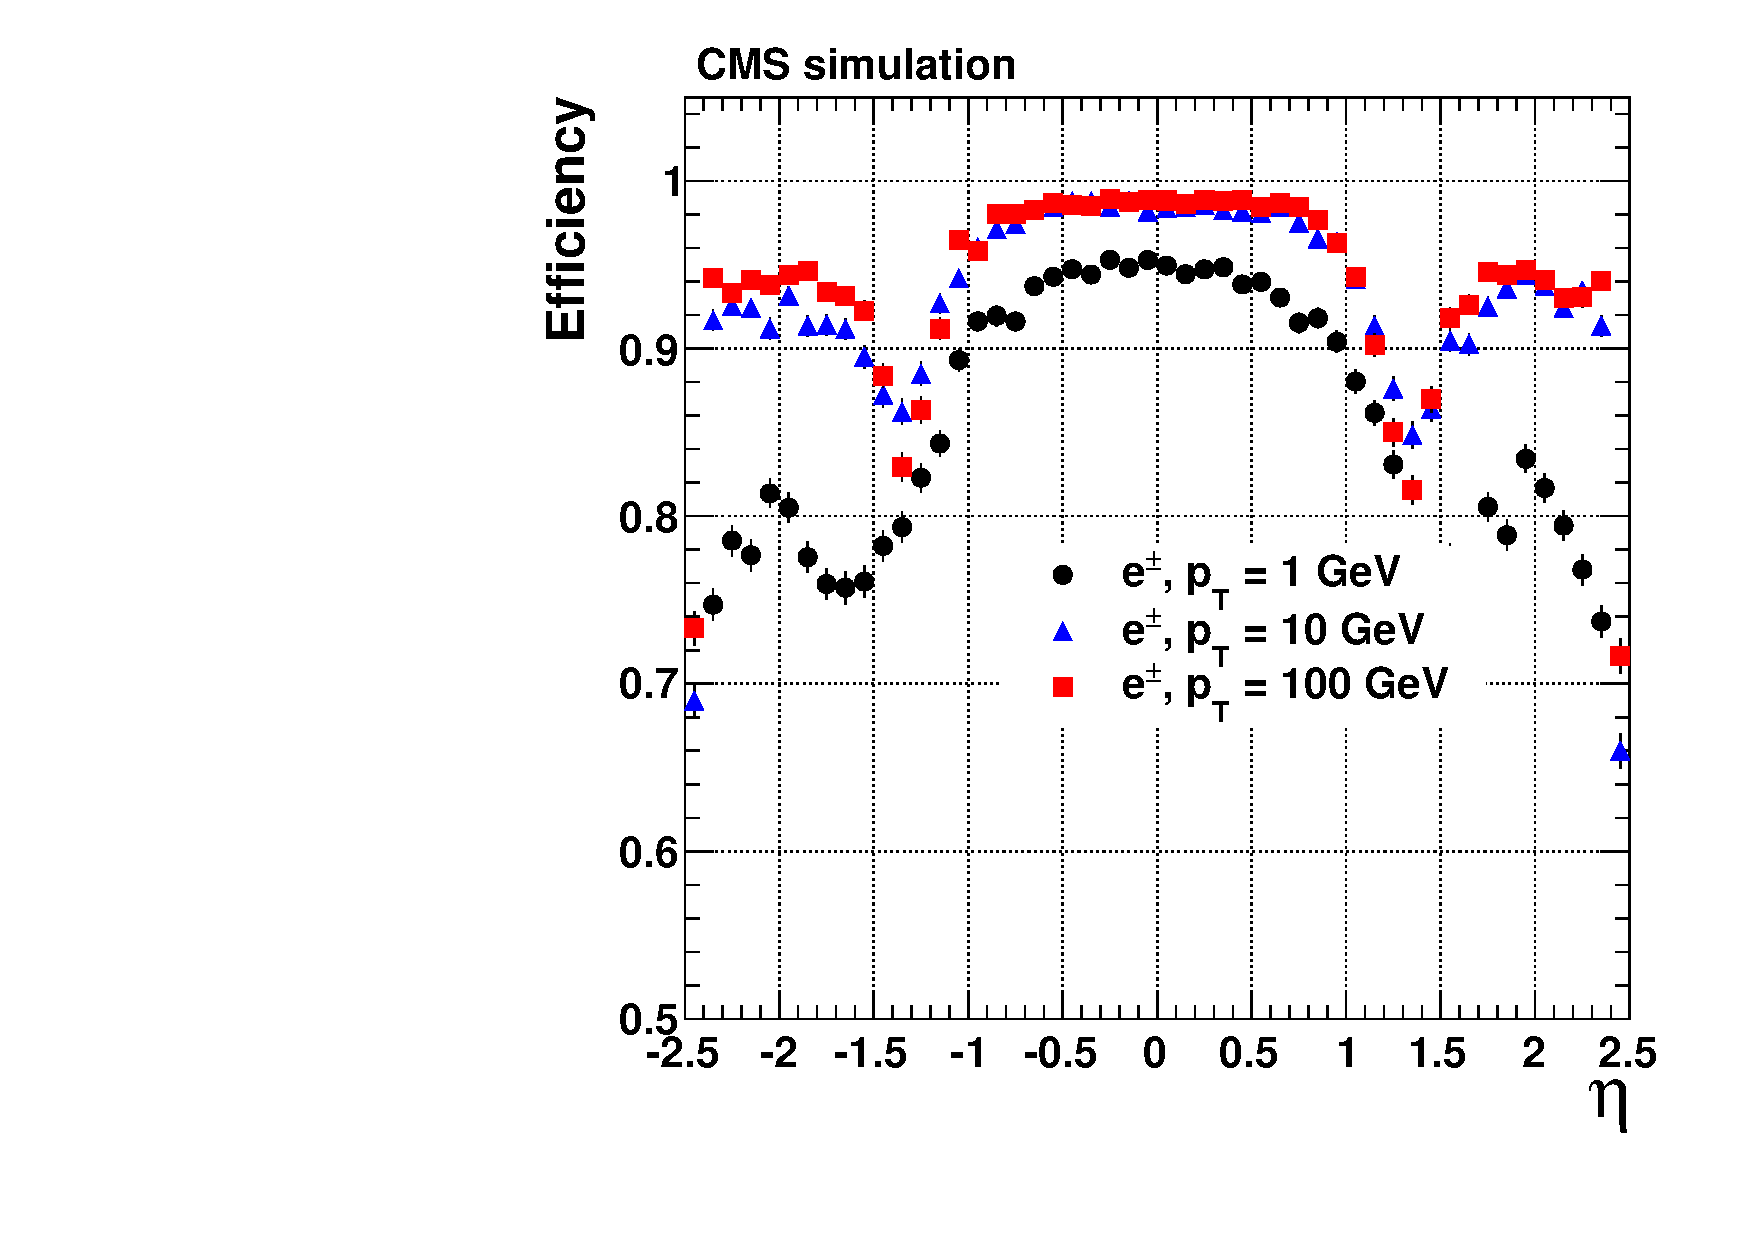
\includegraphics[width=0.30\textwidth]{\chsix/el-efficiencyVsEta.pdf}}
\subfigure[]{\label{fig:track_eff_c}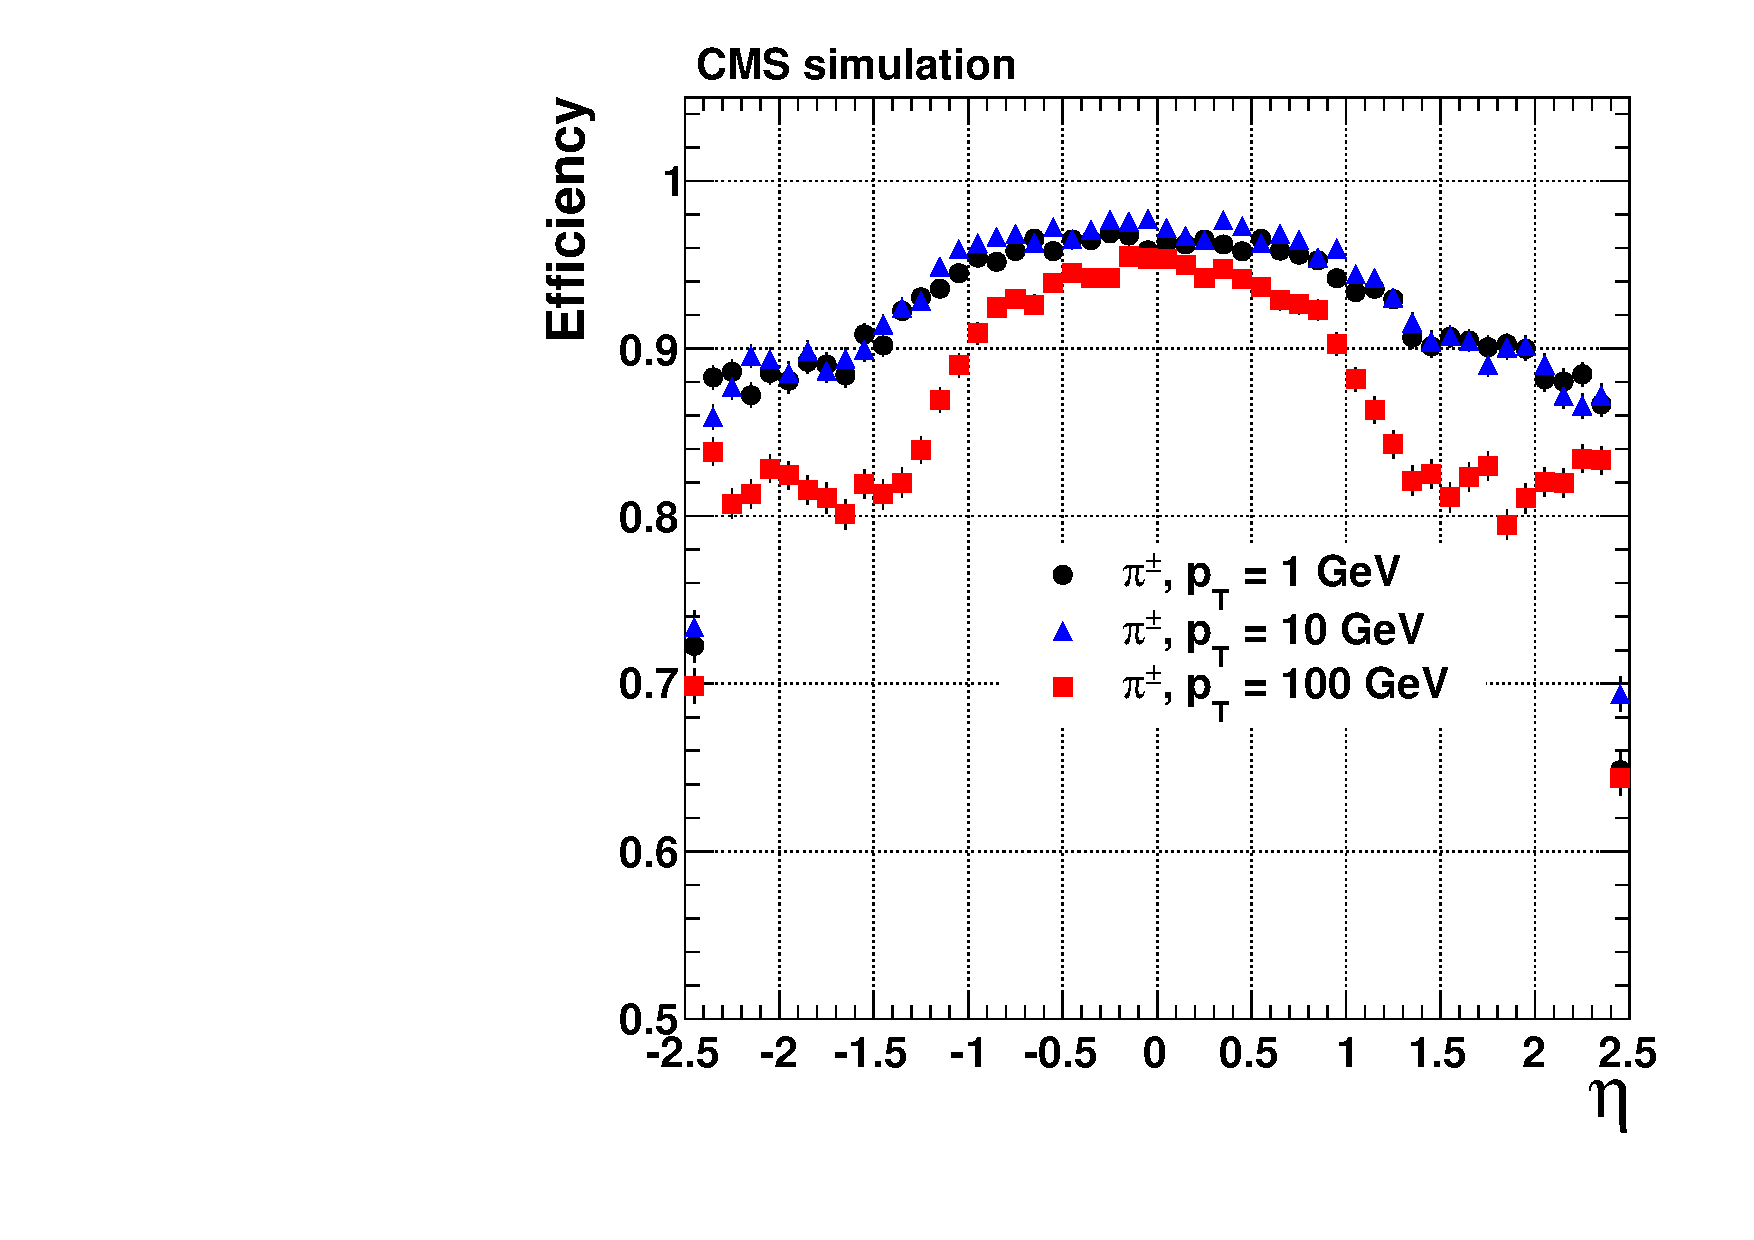
\includegraphics[width=0.30\textwidth]{\chsix/pi-efficiencyVsEta.pdf}}
\caption{Track reconstruction efficiency for simulated muons (a), electrons (b), and pions (c) passing the high-purity quality requirements as a function of $\eta$ and for \pt = 1, 10, and 100 \GeV~\cite{Chatrchyan:2014fea}.}
\label{fig:track_eff}
\end{figure}

\begin{figure}[!htb]
 \begin{center}
  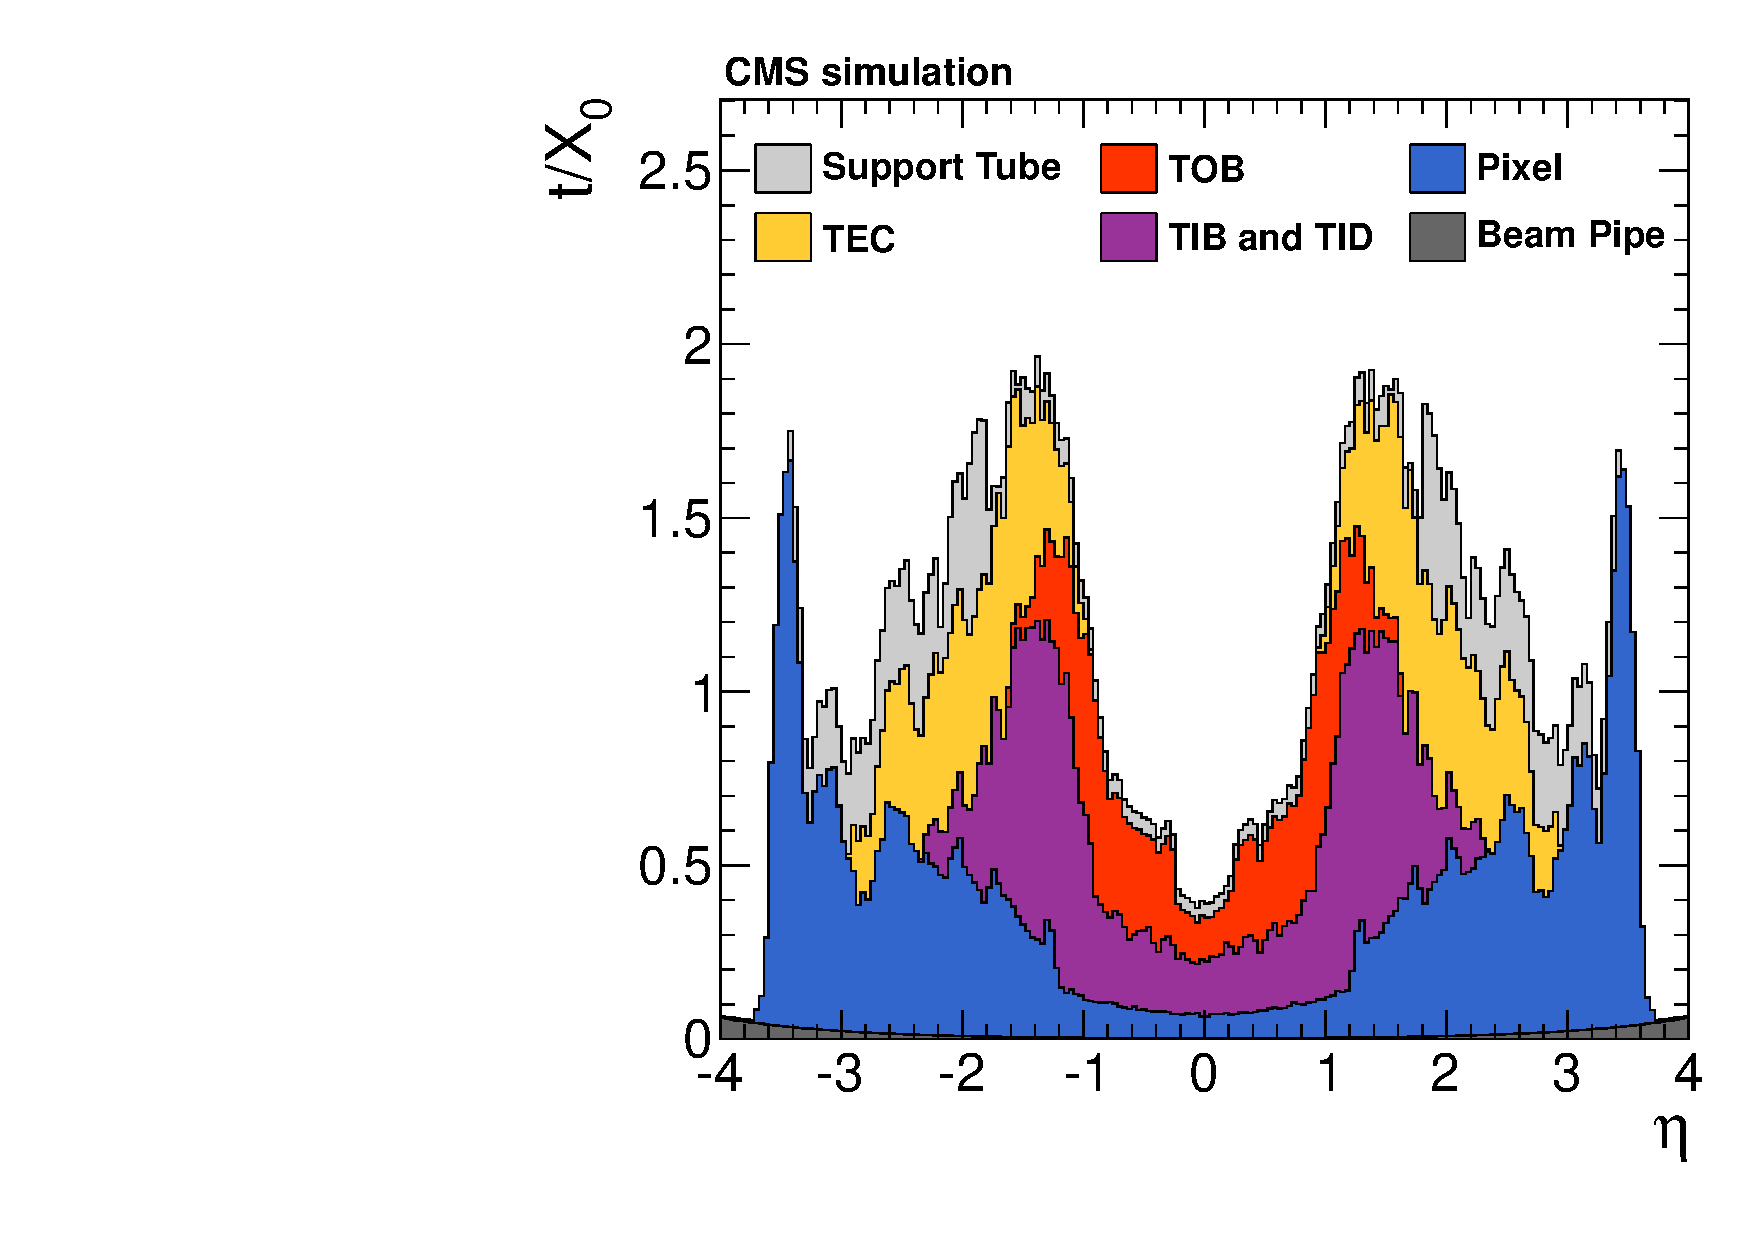
\includegraphics[width=0.45\textwidth]{\chsix/MaterialBudget_RadLengths.pdf}
 \end{center}
 \caption{Material budget of the CMS tracker in units of radiation length $X_0$ as a function of pseudorapidity divided into the contributions of the different sub-detectors~\cite{Chatrchyan:2014fea}.}
 \label{fig:budgetCMStracker}
\end{figure}

In Fig.~\ref{fig:track_mu_rel_a} the transverse momentum resolution for muon tracks with \pt = 1, 10, and 100\GeV is shown. At high transverse momentum (100\GeV), the resolution is 2--3\% up to $|\eta| = 1.6$.
%, but deteriorates at higher $|\eta|$ values, because of the shorter lever arm of these tracks in the $x$-$y$ plane of the tracker.
%The degradation at $|\eta| \sim 1.0$ and beyond is due to the gap between the barrel and the endcap disks, and due to the inferior hit resolution of the last hits of the track measured in TEC ring 7 compared to the hit resolution in TOB layers 5 and 6.
The material of the tracker accounts for 20--30\% of the transverse momentum resolution.
At lower momenta, the resolution is dominated by multiple scattering and its distribution reflects the amount of material traversed by the track.
The resolutions of the track impact parameter in the transverse and longitudinal plane are also shown in Fig.~\ref{fig:track_mu_rel}. At high momentum the transverse impact parameter resolution is fairly constant and is dominated by the hit resolution in the first pixel layer. It is progressively degraded by multiple scattering at lower momenta. The same applies to the longitudinal impact parameter resolution. The improvement of the $z_0$ resolution up to $|\eta| = 0.5$ is due to the charge sharing effects among neighboring pixels.

\begin{figure}[!htb]
\centering
\subfigure[]{\label{fig:track_mu_rel_a}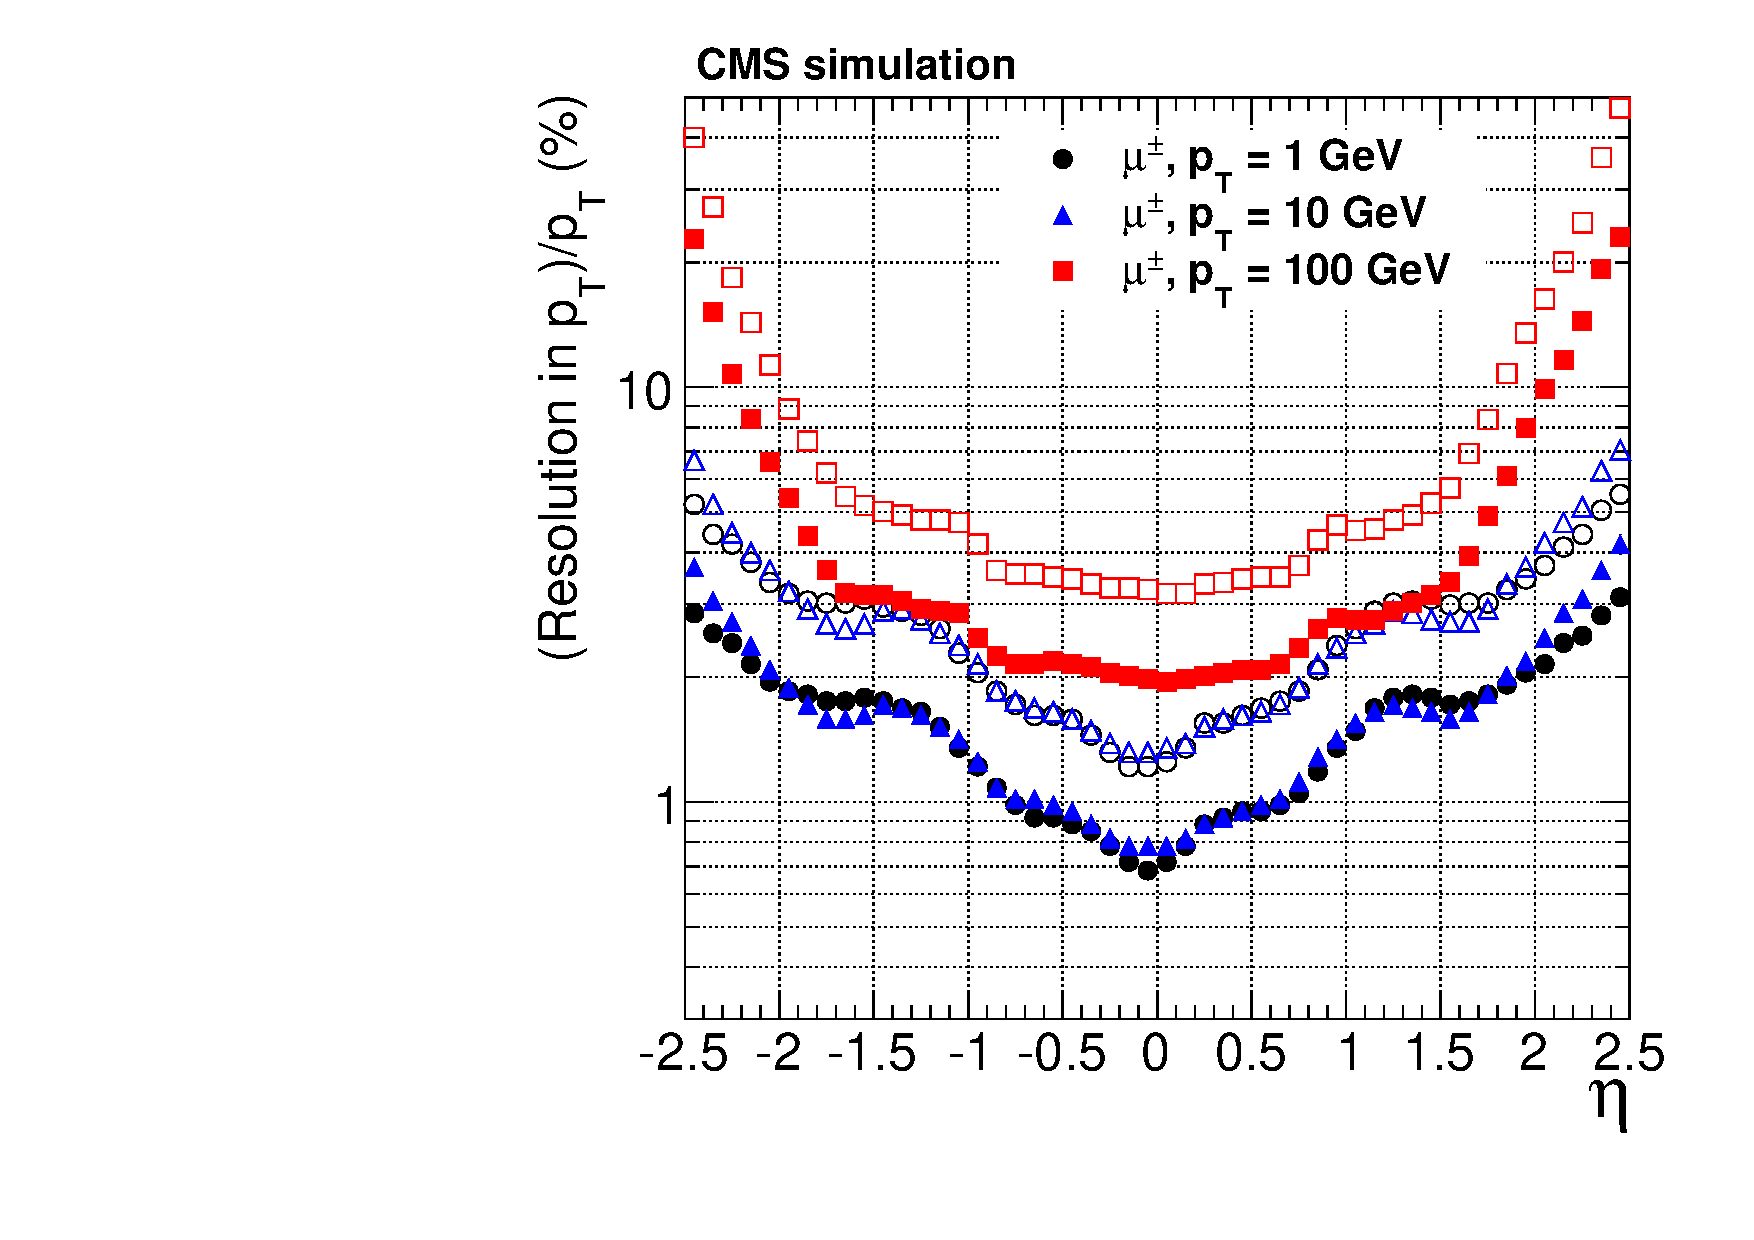
\includegraphics[width=0.30\textwidth]{\chsix/mu-resolutionPtVsEta.pdf}}
\subfigure[]{\label{fig:track_mu_rel_b}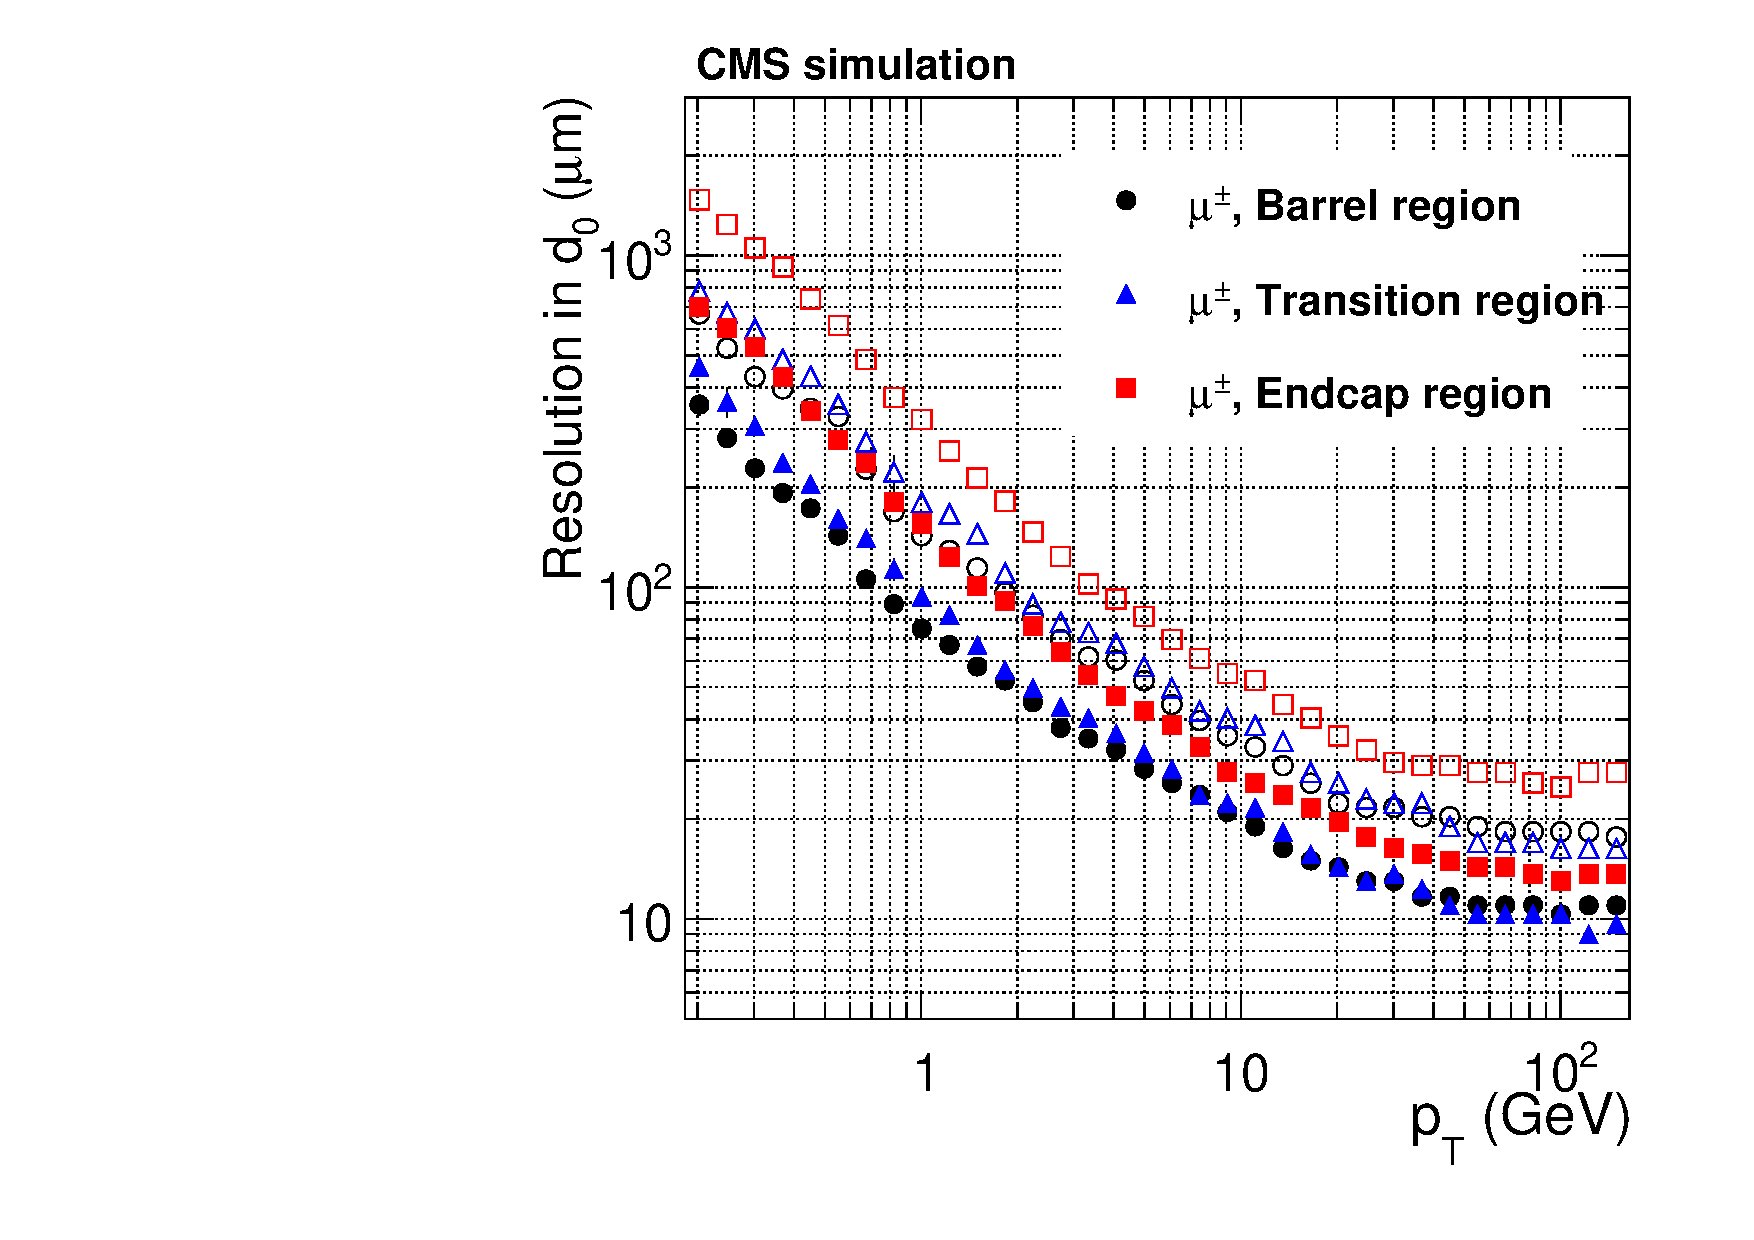
\includegraphics[width=0.30\textwidth]{\chsix/mu-resolutionD0VsPt.pdf}}
\subfigure[]{\label{fig:track_mu_rel_c}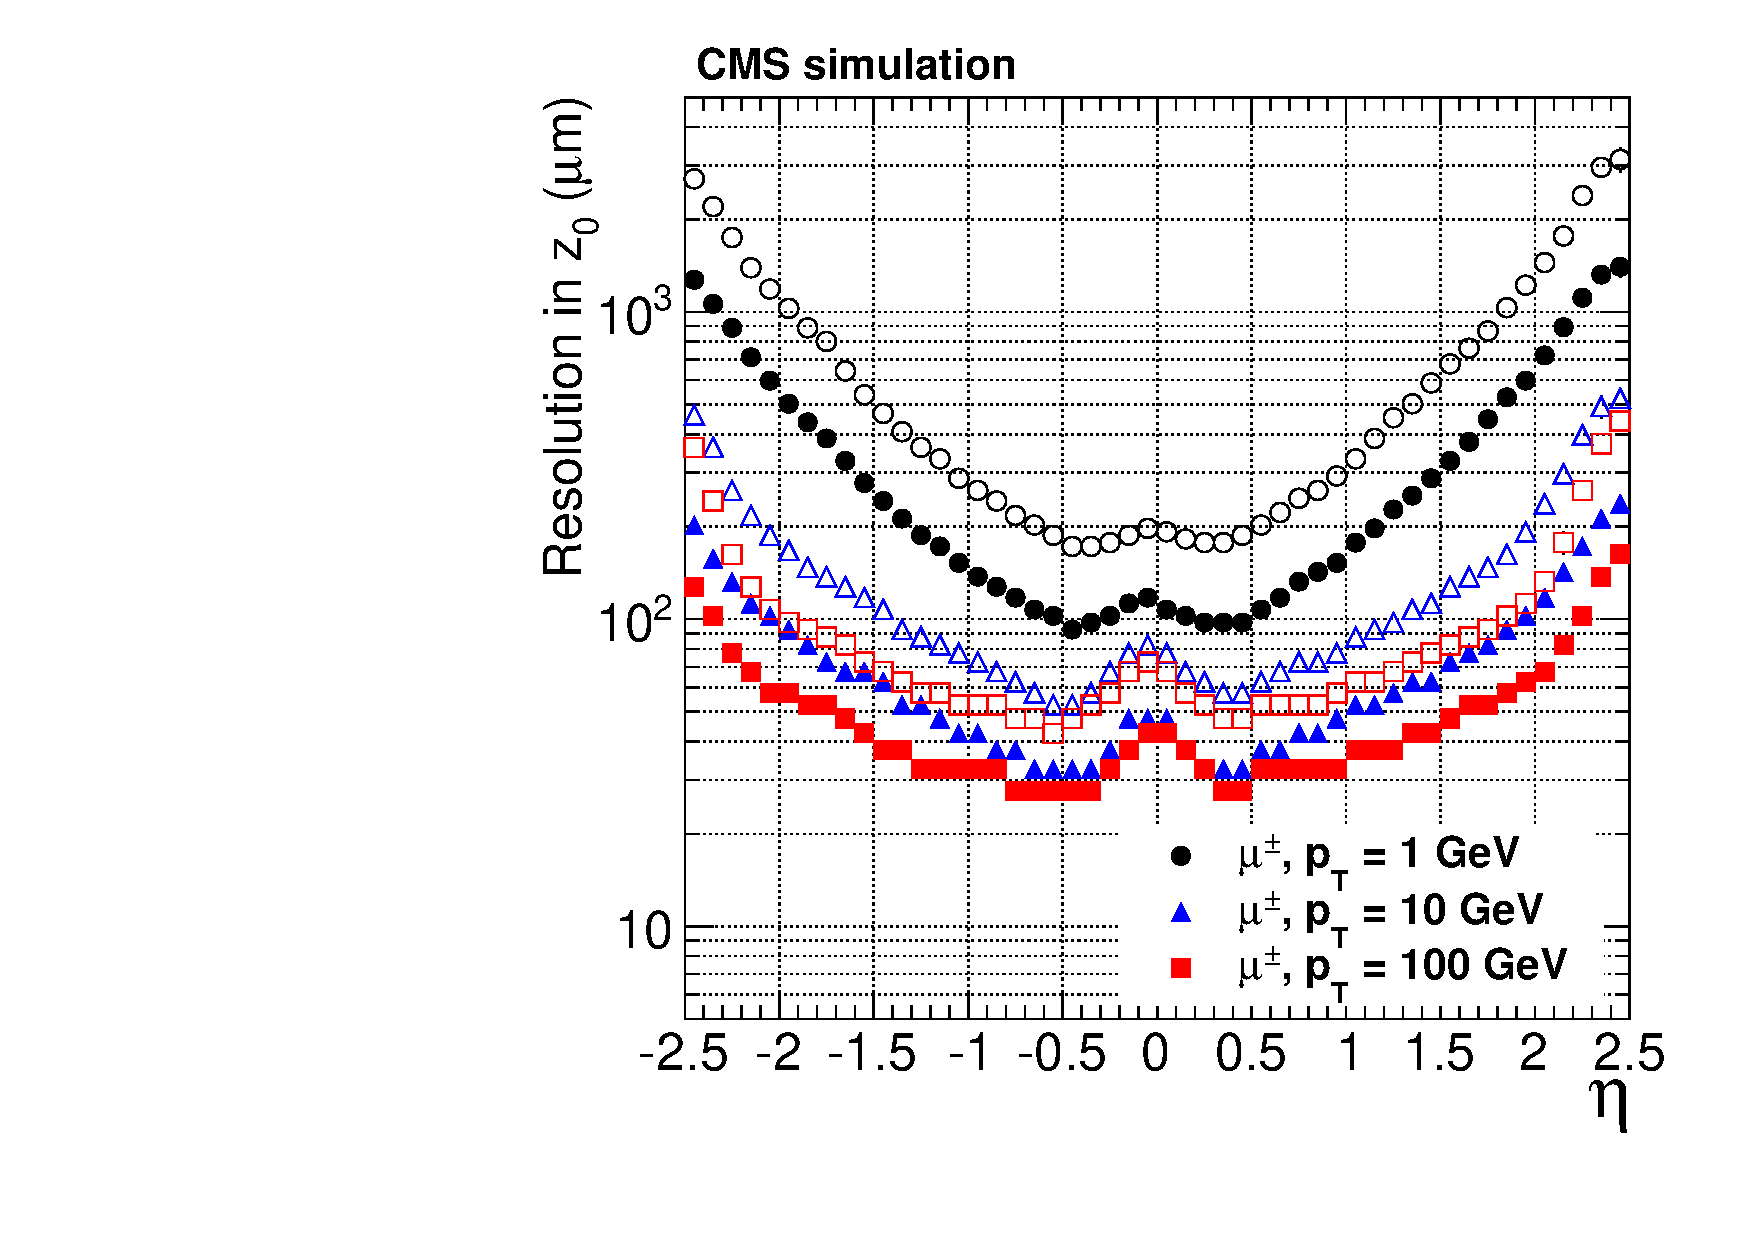
\includegraphics[width=0.30\textwidth]{\chsix/mu-resolutionDzVsEta.pdf}}
\caption{Resolution of track transverse momentum (a), transverse (b) and longitudinal (c) impact parameter for simulated muons passing the high-purity quality requirements as a function of $\eta$ and for \pt = 1, 10, and 100 \GeV~\cite{Chatrchyan:2014fea}.}
\label{fig:track_mu_rel}
\end{figure}

%%%%%%
\subsection{Primary-vertex reconstruction}
%%%%%%

The identification of primary vertices is essential to distinguish the primary vertex associated with the hard interaction from additional pileup vertices that might be present in the event. This became even more important at the highest LHC luminosity reached at the end of 2016 where an average of 25 pp interactions took place simultaneously.\\

In the primary-vertex reconstruction~\cite{Speer:927395}, the measurements of the location and uncertainty of an interaction vertex are computed from a given set of reconstructed tracks. The prompt tracks originating from the primary interaction region are selected based on the transverse impact parameter significance with respect to the beam line, the number of strip and pixel hits, and the normalized track $\chi^2$ from a fit to the trajectory. The selected tracks are then clustered on the basis of their $z$-coordinates at their point of closest approach to the center of the beam spot using a \textit{deterministic annealing} (DA) algorithm~\cite{726788}.
This clustering allows for the reconstruction of any number of pp interactions in the same LHC bunch crossing. Vertices are resolved with separations of about 1\mm, appropriate for a multiplicity of interactions per bunch crossing up to 20, as the longitudinal RMS spread of the luminous region is about 6\cm.

After identifying candidate vertices based on the DA clustering in $z$, those candidates containing at least two tracks are then fitted using an \textit{adaptive vertex fitter}~\cite{0954-3899-34-12-N01}, to compute the best
estimate of vertex parameters, including its $x$, $y$, and $z$ position, and covariance matrix. This algorithm addresses the issue of secondaries and fake tracks in the cluster by iteratively down-weighting the tracks which are not compatible with the fitted common vertex. The primary-interaction vertex, where the hard process of interest takes place, is chosen as the vertex with the highest sum of $\pt^2$ of the clustered tracks.\\
%The first vertex is usually the one corresponding to the collision of interest, where the hard process takes place.
%as well as the indicators for the success of the fit, such as the number of degrees of freedom for the vertex, and weights of the tracks used in the vertex. 

The primary vertex spatial resolution depends on the event topology and on the number of tracks related to the vertex, as shown in Fig.~\ref{fig:vtx_rel}. For minimum-bias events, the resolutions in $x$ and $z$ are, respectively, less than 20\mum and 25\mum, for primary vertices reconstructed using at least 50 tracks. The resolution is better for the jet-enriched sample where tracks have significantly higher mean \pt resulting in better resolution in the track impact parameter, and consequently better vertex resolution. For these events, the resolutions approach 10\mum in $x$ and 12\mum in $z$ for primary vertices using at least 50 tracks.\\

In the analysis described in this work, all events are required to have at least one primary vertex reconstructed within a 24\cm window along the beam axis, with a transverse distance from the nominal pp interaction region
of less than 2\cm.

\begin{figure}[!htb]
\centering
\subfigure[]{\label{fig:vtx_rel_a}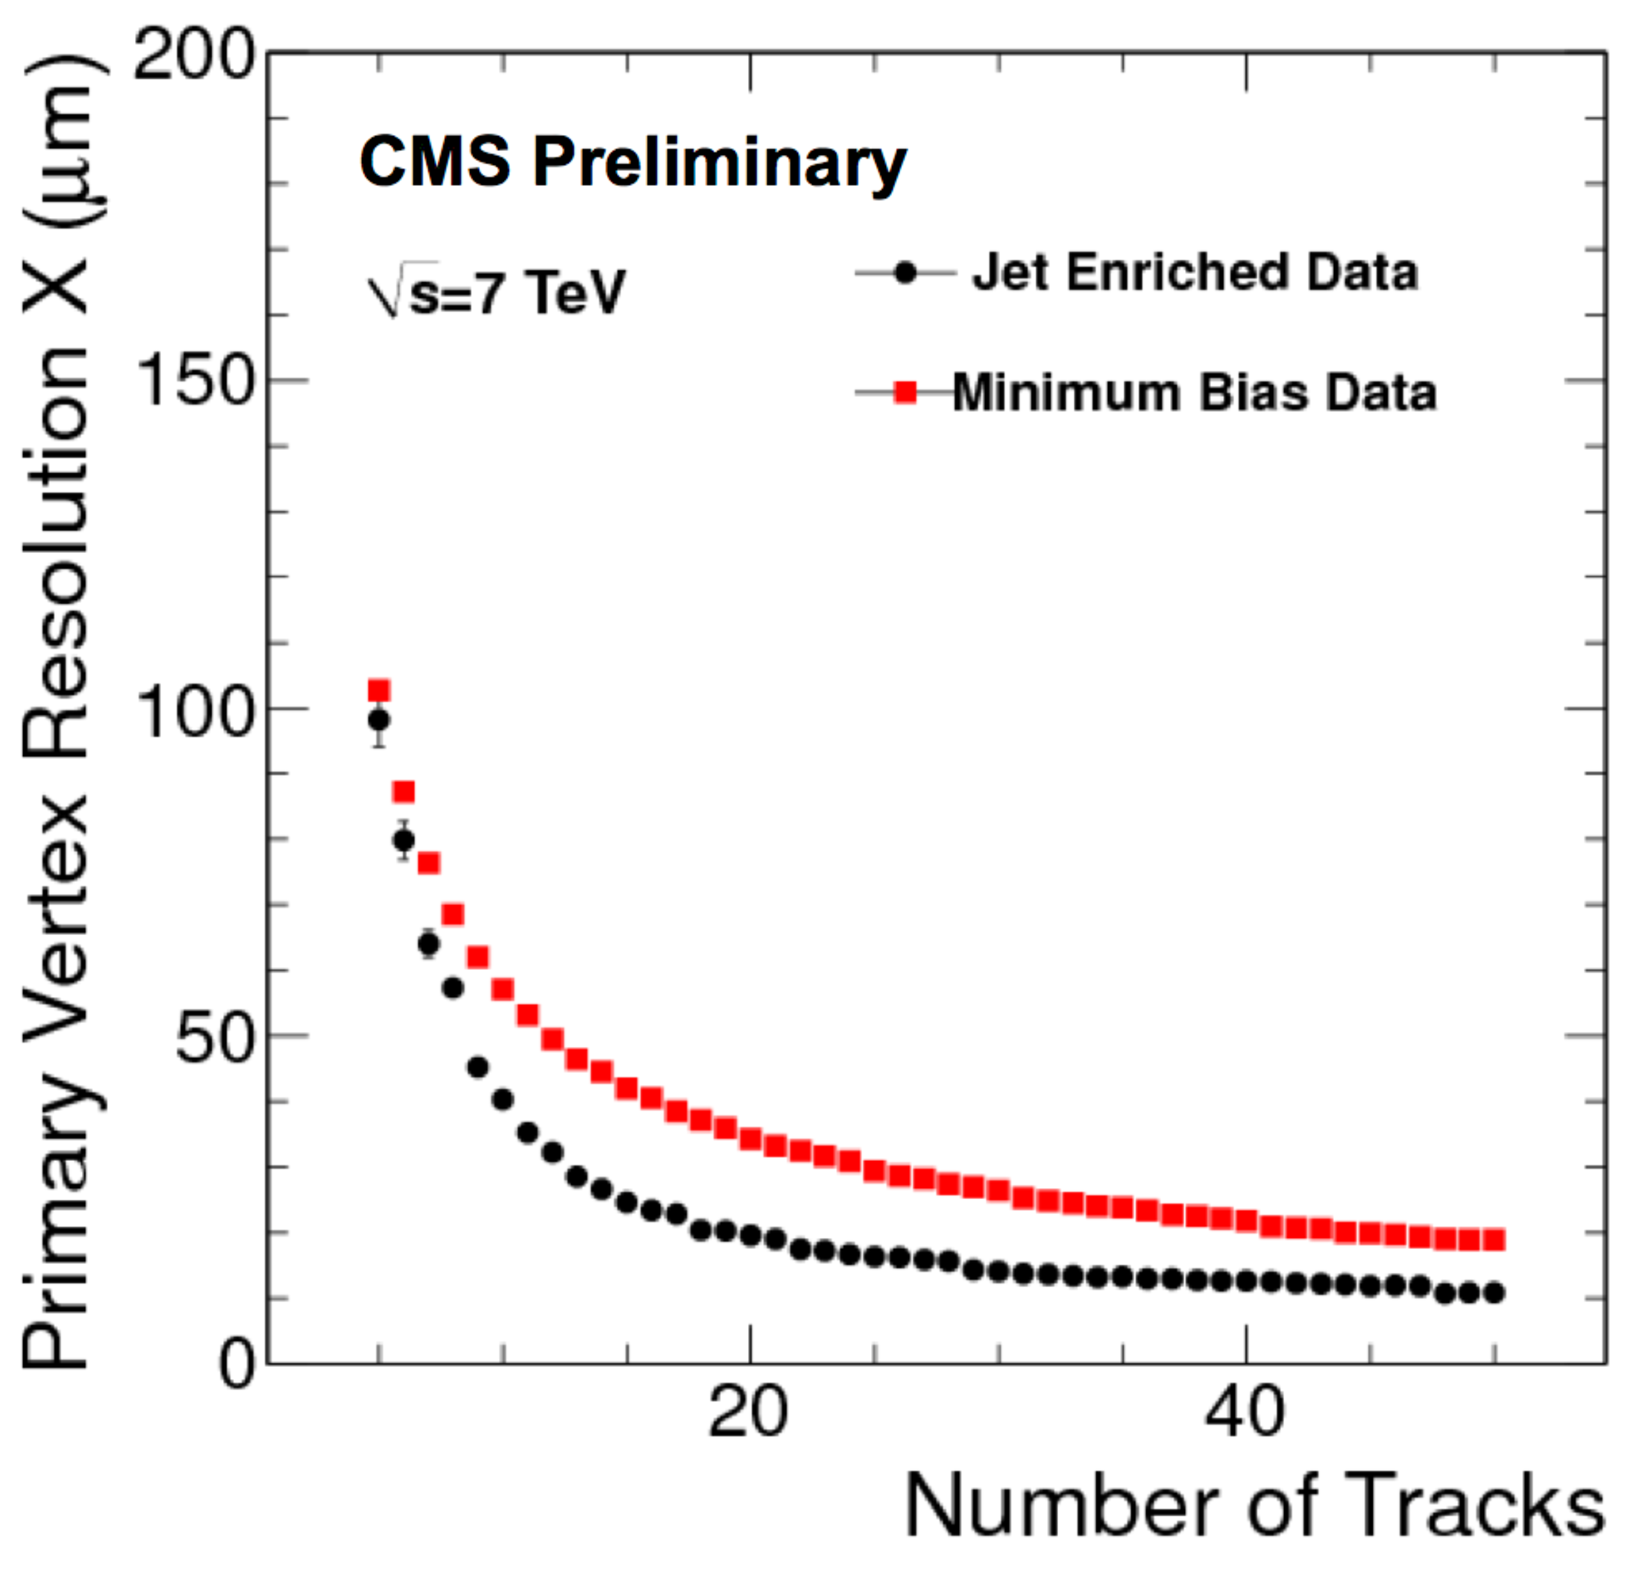
\includegraphics[width=0.45\textwidth]{\chsix/PrimaryVertexResolutionsX.pdf}}
\subfigure[]{\label{fig:vtx_rel_b}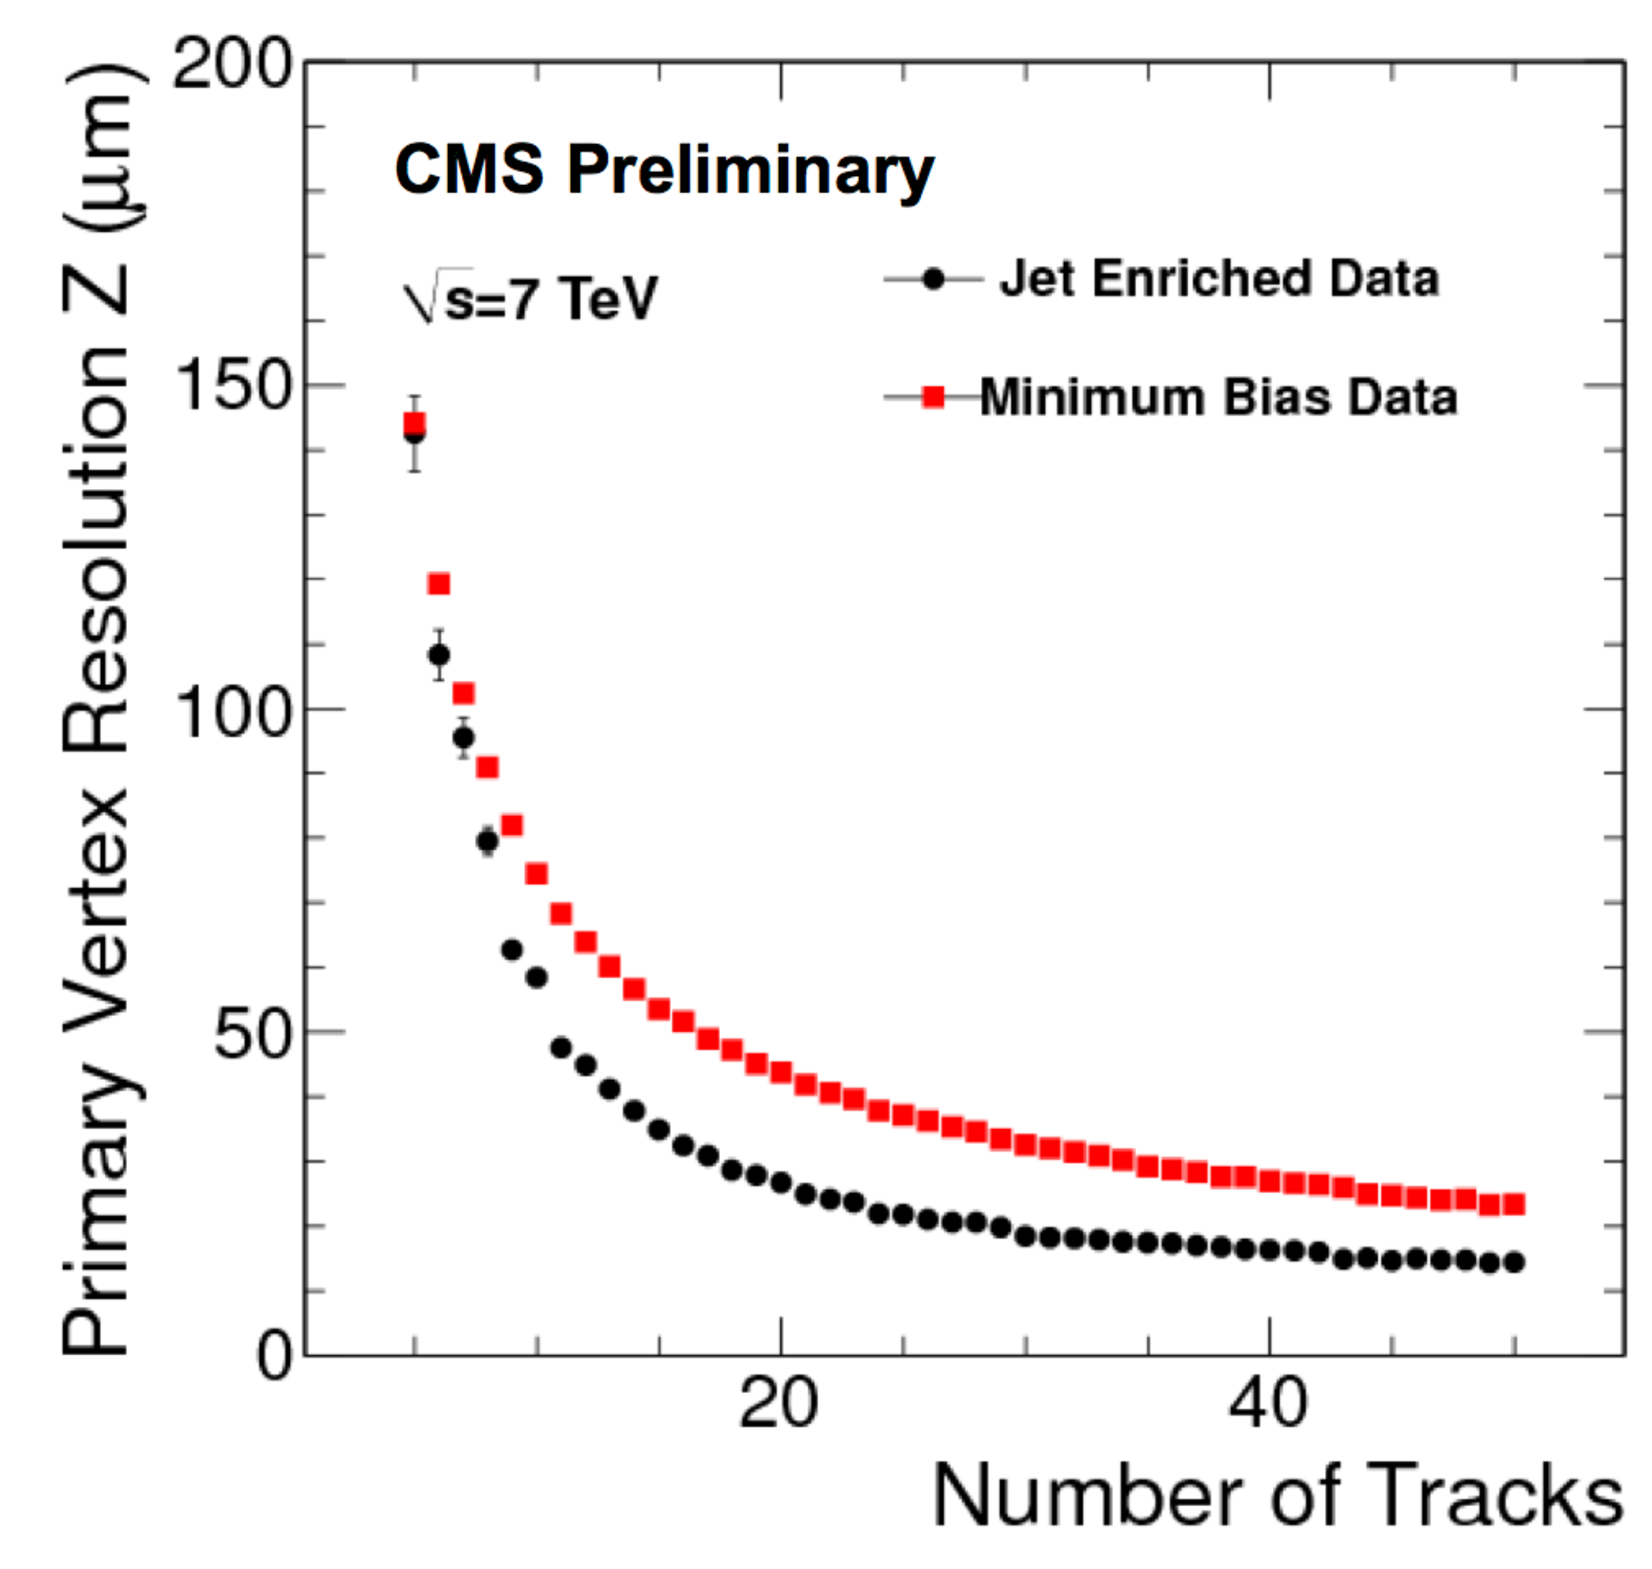
\includegraphics[width=0.45\textwidth]{\chsix/PrimaryVertexResolutionsZ.pdf}}
\caption{Primary-vertex resolution in $x$ (a) and $z$ (b) as a function of the number of tracks at the fitted vertex, for two kinds of events with different average track \pt values. The results in $y$ are almost identical to the one in $x$~\cite{TrkCMSPublicResults}.}
\label{fig:vtx_rel}
\end{figure}
